\documentclass[11pt]{article}

%encoding
\usepackage[T1]{fontenc}
\usepackage[utf8]{inputenc}
\usepackage{lmodern}

%language
\usepackage[english]{babel}

%paper and text body handling
\usepackage{geometry}
\usepackage{fancyhdr} %Headers and footers
\usepackage{setspace}
\usepackage{lettrine}
\usepackage{glossaries}

%graphics
\usepackage{graphicx}
\graphicspath{{Images/}{./}}
\usepackage[format = plain, labelfont = {bf, it}, textfont = it]{caption}%font settings for captions
\usepackage{xcolor}
\usepackage{pdfpages}
\usepackage{subcaption}
\usepackage{tikz}

%code
%\usepackage{minted}

%math
\usepackage{amsmath}%math
\usepackage{amssymb}%
\usepackage{amsfonts}%
\usepackage{amsthm}%theorems
\usepackage{aligned-overset}
\usepackage{siunitx}
\usepackage{cancel}
\usepackage{braket}
\usepackage{bm}
\usepackage{diffcoeff}
% Use the correct ds in diffs
\difdef{f,s,c}{}{
  op-symbol = \mathrm{d},
}
\difdef{f,s}{f}{
	op-symbol = \delta,
}

%bibliography
\usepackage{csquotes}%for biblatex
\usepackage[
   style = numeric,
   sorting = none,
   date = iso,
   seconds = true
]{biblatex}

%links
\usepackage[colorlinks=true,
            linkcolor=red,
            urlcolor=blue,
            citecolor=gray]{hyperref}

%todo
\usepackage[colorinlistoftodos]{todonotes}

\input{mathCommands}
%text
\makeatletter
   \newlength{\textSize}
   \setlength{\textSize}{\f@size pt}
\makeatother
\setlength{\parindent}{0pt}             % No indentation on new paragraph
\setlength{\parskip}{\textSize}         % Blankline on new paragraph
\setstretch{1.15}


%paper and text body
\geometry{
   a4paper,
   centering,
}


%lettrine settings
\setcounter{DefaultLines}{3}


\newacronym{pml}{PML}{Perfectly Matched Layer}

%bibliography
\addbibresource{sources.bib}

\title{Inverse design of quantum acoustic devices}
\author{David Hambr\ae{}us}
\date{\textit{\today}}

\begin{document}

\maketitle

\todo[inline]{Todonotes are organized as follows:}
\todo[inline]{General comment / question}
\todowrt{Things that could be done now, no further
simulations/consultation needed}
\tododec{Things that could be done now but I am not sure if I should, or
how to do it}
\todoblk{Things that can't be done yet because they depend on other
things, e.g.\ results}
\todocit[inline]{Citation needed}

\listoftodos[List of Todos]

\tableofcontents

\printglossaries{}

\newpage

\section{Introduction}

\tododec{Introduction to quantum acoustics\ldots I need to read more
literature I think}

Conventionally, when designing these components, the designer comes up with a
design through intuition and parametrizes it with a couple of parameters.
For example they may believe that a structure with periodically placed circular
holes should yield a device that performs the desired function.
% TODO: She? I wrote he first but that will only reinforce the stereotype that
% the are no women in nano science.
The parameters that are unknown might then be the distance between neighbouring
holes and the radius of the holes.
To find the optimal device they would then systematically test parameter values
to see which give the best performance in a simulation of the device.
This brute force method of design limits the possible number of parameters to a
very small number.
If there are 10 different values to test for each parameter, the even 6
parameters would require 1,000,000 simulations.
One can of course use smarter optimization algorithms like bayesian optimization
\todocit{cite something, check Ida's thesis maybe}
or particle swarm optimization
\todocit{cite the thing the danish guys cited}
to decrease the number of simulations needed, but it will still be of the same
order.

A different approach that has been gaining some popularity is
\emph{inverse design with adjoint simulation}.
\todocit{maybe cite \emph{inverse design in nanophotonics}}
The idea is that if the gradient of the figure of merit
with respect to the parameters can be calculated, then we can use gradient based
optimization methods, which converge much faster, even if the number of
parameters is very large. With these methods, one hopes to be able to search
among a much more general class of designs for the optimal one.
% Su? Isn't it Jelena?
\citeauthor{spins2019} has developed software that successfully uses inverse design for
nanophotonic devices \cite{spins2019}.

With this thesis, we explore the possibility of extending this paradigm to
acoustic devices. In order to do so, we attempt to design a phononic beam
splitter.

\subsection{Thesis outline}

\section{Theory}

Maybe some mechanics theory? Linear elastic material etc.
Maybe also mode shape and what the waveguides / mode that we are designing for
is? should that be here? It doesn't really fit in the method section I think...
And more generally how waveguides work?

\subsection{Acoustic waves and waveguides}

In order to efficiently model the deformation and stresses in a solid material,
a linear elasticity model is often assumed.
For small deformations, solid materials obey Hooke's law which in it's full form
looks like
\[
	\sigma_{ij} = C_{ijkl} \epsilon_{jl}
\]
where $\sigma$ is the stress tensor, $C$ the elasticity tensor which is a
property of the material, and 
$\epsilon \defeq \nabla \vec u + (\nabla \vec u)^T$
is the strain tensor.
This equation is linear in $\vec u$, hence the name \emph{linear} elasticity.
Using this and newtons equations of motion, the equation governing the dynamics
is obtained:
\[
	\rho \ddot{\vec{u}} = \nabla \cdot \sigma + \vec F.
\]
where $\rho$ is the density, $\vec{u}$ is the displacement and $\vec F$ is the
externally applied force.
\tododec{Proper derivation for equation below? It is relatively
straightforward but requires some effort}
Assuming a time harmonic solution
$\vec u(\vec x, t) = \vec u(x) e^{i \omega t}$ and plugging this into
the governing equations yields
\todo[inline]{
	Minus sign here? Inconsistent with 3.21 in Chan's PhD thesis, but that is
	not consistent with itself... (3.19). Comsol has the minus sign, so probably
	Chan's equation has a typo.
}
\begin{equation}\label{eq:gov_eq}
	-\rho \omega^2 u_i = \partial_j C_{ijkl} \partial_k u_l + F_i
\end{equation}
written in index notation for clarity. 

\todowrt{
With no external forces we get traveling modes=eigenvalues.
Explain how and why periodicity means only certain modes can propagate.
Good resource in Chan's thesis, or maybe solid state physics book?
% Bloch state / Bloch's theorem
}

\subsection{Adjoint Simulation}

\todowrt{Introduce the point of inverse design, that there is an objective
function / figure of merit and that we want to find the derivative of it w.r.t
the material parameters.}

\tododec{Derive the general case: governing eq $Au = b$}

\tododec{Derive specific case (with functional analysis):
	borrowing heavily from the mathy notes is possible.
	Derivation is theoretically possible without specifying that the objective function
	is an overlap integral, only
	using equation~\eqref{eq:gov_eq},
	but the equations would be \emph{a lot} longer and more abstruse,
	so I don't think that it is a good idea.
}

\subsection{Optimization Algorithms}

\tododec{General paragraph on the benefits of gradient based
optimization algorithms vs other algorithms? And general overview of the
optimization process: simulate -- compute gradient -- step}

\todowrt{Paragraph describing regular gradient descent}

\todowrt{Paragraph describing the ADAM algorithm}

\section{Methods}

The aim of this thesis is to use inverse design to find a phononic beamsplitter,
a task that can be divided into three parts: 
First, some definitions of what
should be designed and what constitutes a ``good'' design needs to be made.
Second, we need a way to calculate the gradient of the ``goodness'' with respect
to the design.
And lastly, we need a gradient based optimization algorithm to find the optimal
design.
All of this will be described in this chapter.

\subsection{Design}

The device design to be optimized can be seen in figure~\ref{fig:bs-design}

\begin{figure}[htpb]
	\centering
	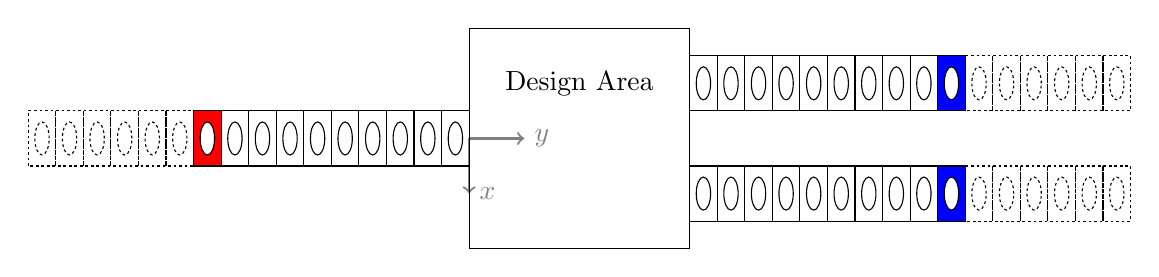
\begin{tikzpicture}[scale=0.7]
	\def \a{0.5}
	\def \w{1.0}
	\def \hx{0.13}
	\def \hy{0.3}
	\def \designx{4.0}
	\def \designy{4.0}
	\def \outputh{1.0}
	\def \nunitcells{16}
	\def \nnonpmls{10}

	% Coordinate system
	\draw[gray, thick, ->] (0,0) -- (0,-1) node [anchor=west] {$x$};
	\draw[gray, thick, ->] (0,0) -- (1,0) node [anchor=west] {$y$};

	% Input waveguide
	\begin{scope}[dash=on 1pt off 1pt phase 0pt]
		\foreach \ix [parse=true] in {-\nunitcells,...,-\nnonpmls-1} {
			\draw (\ix*\a, -0.5*\w) rectangle (\ix*\a + \a, 0.5*\w);
			\draw (\ix*\a + 0.5*\a, 0) circle [x radius=\hx, y radius=\hy];
		}
	\end{scope}
	\foreach \ix in {-\nnonpmls,...,-1} {
		\draw (\ix*\a, -0.5*\w) rectangle (\ix*\a + \a, 0.5*\w);
		\draw (\ix*\a + 0.5*\a, 0) circle [x radius=\hx, y radius=\hy];
	}
	\draw[fill=red] (-\nnonpmls*\a, -0.5*\w) rectangle (-\nnonpmls*\a+\a, 0.5*\w);
	%\node at (-\nnonpmls*\a + 0.5*\a, 0.5*\w) [anchor=south, red] {forward load};
	\draw[fill=white] (-\nnonpmls*\a + 0.5*\a, 0) circle [x radius=\hx, y radius=\hy];

	% Design area
	\draw (0, -\designx / 2) rectangle (\designy, \designx / 2);
	\node at (\designy / 2, 1) {Design Area};

	% Output waveguide
	\foreach \ix [parse=true] in {0, ..., \nnonpmls-1} {
		\draw (\designy + \ix*\a, \outputh - 0.5*\w) rectangle 
			  (\designy + \ix*\a + \a, \outputh + 0.5*\w);
		\draw (\designy + \ix*\a + 0.5*\a, \outputh)
			circle [x radius=\hx, y radius=\hy];

		\draw (\designy + \ix*\a, -\outputh - 0.5*\w) rectangle 
			  (\designy + \ix*\a + \a, -\outputh + 0.5*\w);
		\draw (\designy + \ix*\a + 0.5*\a, -\outputh)
			circle [x radius=\hx, y radius=\hy];
	}
	\begin{scope}[dash=on 1pt off 1pt phase 0pt]
		\foreach \ix [parse=true] in {\nnonpmls, ..., \nunitcells-1} {
			\draw (\designy + \ix*\a, \outputh - 0.5*\w) rectangle 
				  (\designy + \ix*\a + \a, \outputh + 0.5*\w);
			\draw (\designy + \ix*\a + 0.5*\a, \outputh)
				circle [x radius=\hx, y radius=\hy];

			\draw (\designy + \ix*\a, -\outputh - 0.5*\w) rectangle 
				  (\designy + \ix*\a + \a, -\outputh + 0.5*\w);
			\draw (\designy + \ix*\a + 0.5*\a, -\outputh)
				circle [x radius=\hx, y radius=\hy];
		}
	\end{scope}
	\draw[fill=blue] (\designy + \nnonpmls*\a - \a, \outputh-0.5*\w) rectangle
		(\designy + \nnonpmls*\a, \outputh + 0.5*\w);
	\draw[fill=white] (\designy + \nnonpmls*\a - 0.5*\a, \outputh) circle [x radius=\hx, y radius=\hy];
	\draw[fill=blue] (\designy + \nnonpmls*\a - \a, -\outputh-0.5*\w) rectangle
		(\designy + \nnonpmls*\a, -\outputh + 0.5*\w);
	\draw[fill=white] (\designy + \nnonpmls*\a - 0.5*\a, -\outputh) circle [x radius=\hx, y radius=\hy];


\end{tikzpicture}

	\caption{
		Device design to be optimized.
		At the red line, a wave traveling right is excited.
		On the blue unit cells is where the output is measured.
		The dashed unit cells are \gls{pml}
	}
	\label{fig:bs-design}
\end{figure}

\subsubsection{Level-set}

\todowrt{Description of what level-set is: A way of storing a boundary between
two regions; and how it works: Signed distance function}

\todowrt{Description of it's advantages: Easily evolved (level-set equation), no
connectivity issues, see level-set book}

\tododec{Write about how I use it? This feels like it should come after I've
talked about computing the derivative.}

\subsubsection{Objective function}

\tododec{Maybe I'll only mention that $f$ is an integral of the displacement
	field in the theory and here give the specific formula:
}
\begin{equation}
	f_\text{obj} = \int_{\Omega_1} \vec{m_1}^*(\vec{x}) \vec{u}(\vec{x})
	\dl{x} + \int_{\Omega_2} \vec{m_2}^*(\vec{x}) \vec{u}(\vec{x})
\end{equation}

\tododec{Paragraph about pure part of objective function, enforcing the minimum
feature size}

\subsection{Adjoint Simulation}

\tododec{Give the explicit formula for the gradient now that the objective
function has been fully defined}

\subsection{Optimization}

\tododec{Describe what optimization algorithm was used, as well as how this
	changed during the simulation. E.g.\ first 200 iterations ADAM; next ADAM
	but with sigmoid function application; sigmoid + feature size; and finally level-set.
}

\section{Results}

\section{Discussion}

\section{Conclusions}

\printbibliography{}

\end{document}
